\documentclass[12pt,a4paper]{article}

\usepackage{tikz,cancel,amsmath,amssymb,amsfonts,setspace,soul,nicefrac}
\usetikzlibrary{patterns,decorations}

\title{Fundamentos da Física III}
\author{Yuri Santos Silva}
\date{26, Fev. de 2025}

\begin{document}
  \maketitle
  \pagenumbering{gobble}

  1) Uma onda senoidal que se propaga em uma corda é mostrada duas vezes na 
  figura abaixo, antes e depois que o pico A, se desloque em uma distância 
  $d= 6,0$ cm no sentido positivo de um eixo x em $t = 4,0$ s (errata). A distância entre as 
  marcas do eixo horizontal são de 15 cm, a altura H=8,0 mm. Se a equação da 
  onda é formada por $y(x,t)=y_m \sin(kx - \omega t)$. Determine:

  \[
    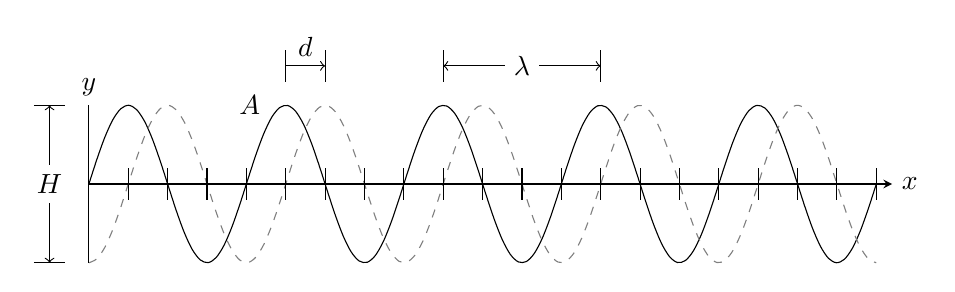
\begin{tikzpicture}[domain=0:10]
      \draw[] plot[samples=100,smooth]({\x},{sin(\x * pi r)});
      \draw[dashed,gray] plot[samples=100,smooth]({\x},{-cos(\x * pi r)});

      \draw[] (0,0) -- (10,0);
      \draw[] (0,-1) -- (0,1) node[anchor=south] {$y$};
      \draw[->,>=stealth] (0,0) -- (10.2,0) node[anchor=west] {$x$};

      \foreach \x in {0.5,1,...,10}
        \draw (\x,.2) -- (\x,-.2);

      \draw[<->] (-.5,-1) -- (-.5,1) node[midway,fill=white] {$H$};
      \draw (-.7,1) -- (-.3,1);
      \draw (-.7,-1) -- (-.3,-1);
      
      \draw[->] (2.5,1.5) -- (3,1.5) node[anchor=south,midway] {$d$};
      \draw[] (2.5,1.7) -- (2.5,1.3);
      \draw[] (3,1.7) -- (3,1.3);

      \draw[<->] (4.5,1.5) -- (6.5,1.5) node[midway,fill=white] {$\lambda$};
      \draw[] (6.5,1.7) -- (6.5,1.3);
      \draw[] (4.5,1.7) -- (4.5,1.3);

      %\draw[<->] (1.5,-1.5) -- (3.5,-1.5) node[fill=white,midway] {T};
      %\draw[-] (1.5,-1.3) -- (1.5,-1.7);
      %\draw[-] (3.5,-1.3) -- (3.5,-1.7);
      
      %\draw[<->] (5.5,-1.5) -- (7.5,-1.5) node[fill=white,midway] {k};
      %\draw[-] (5.5,-1.3) -- (5.5,-1.7);
      %\draw[-] (7.5,-1.3) -- (7.5,-1.7);

      \node[anchor=east] at (2.3,1) {$A$};

    \end{tikzpicture}
  \]

  Dados:
  \vspace*{.2cm}

  \(
    \left\{
        \begin{array}{cclcl}
          d & = & 6,0\ \text{cm} & = & 0,06\ \text{m} \\
          H & = & 8,0\ \text{mm} & = & 0,008\ \text{m} \\
          x_i & = & 15\ \text{cm} & = & 0,15\ \text{m} \\
          T & = & 4,0\ \text{s}
        \end{array}
    \right.
  \)
  \vspace*{.5cm}

  a) A amplitude de $y_m$;
  \[
        y_m = \frac{H}{2} = \frac{8,0\ \text{mm}}{2} = 4,0\ \text{mm}
  \]

  b) O número de onda. \\
  Comprimento de onda é a distância de uma crista (ponto máximo) até outra.
  Sabe-se que cada crista tem 0,15 m e percorre 4 demarcações de $x$.
  \[
    \lambda = 4 \cdot 0,15\ \text{m} = 0,60\ \text{m}
  \]

  Assim podemos calcular o número de onda normalmente:
  \[
    k = \frac{2\pi}{\lambda} = \frac{2\pi}{0,60\ \text{m}} = 
    \frac{20\pi}{6\ \text{m}} = \frac{10\pi}{3} = 3,\bar{3}\pi\ \text{rad/m}
  \]

  c) A frequência angular. \\
  \st{Não nos foi dado nenhuma medida de tempo, ou relacionada, logo não é possível achar o resultado
  numérico dessa questão.}
  \[
    \omega = \frac{2\pi}{4} = \frac{\pi }{2}\ \text{rad/s}
  \]

  \vspace*{.5cm}

  d) O sinal que precede $\omega$.\\
  A onda foi transladada no eixo x para a direita, o que implica em um sinal negativo.
  \vspace*{.5cm}

  e) Elabore o gráfico da onda, na posição x=2 cm em função de um tempo. \\
  Equação: 
  \[
    y(0,02;t) = 4\cdot \sin\left[\frac{10\pi}{3}(0,02) - \frac{\pi}{2}(t)\right] \ \text{mm}
  \]
  \[
    y(0,02;t) = 4\cdot \sin\left[\frac{\pi}{15} - \frac{\pi}{2}(t)\right] \ \text{mm}
  \]

  Ponto inicial: 
  \[
    4\cdot \sin \left( \frac{\pi}{15} \right) \approx 4\cdot \sin (0,21) 
    \approx 4\cdot0,21 = 0,84\ \text{mm}
  \]

  Interseção com o eixo x:
  \[
    \frac{\pi}{15} = \frac{\pi}{2} (t) \implies \frac{1}{15}(2) = t = \frac{2}{15} + \pi k : k \in \mathbb{Z}
  \]

  Segundo ponto para saber a direção: Escolhemos um menor que a interseção com eixo x.
  \[
    t\left(\frac{2}{100};\nicefrac{1}{15}\right) = 4 \cdot \sin \left[\frac{\pi}{15} - \frac{\pi}{2}
    \left( \frac{1}{15} \right)\right] = 4 \sin \left(\frac{2\pi - \pi}{30}\right)
    = 4\sin\left(\frac{\pi}{30}\right) \approx 0,4\ \text{mm}
  \]

  Podemos plotar o gráfico:

  \[
    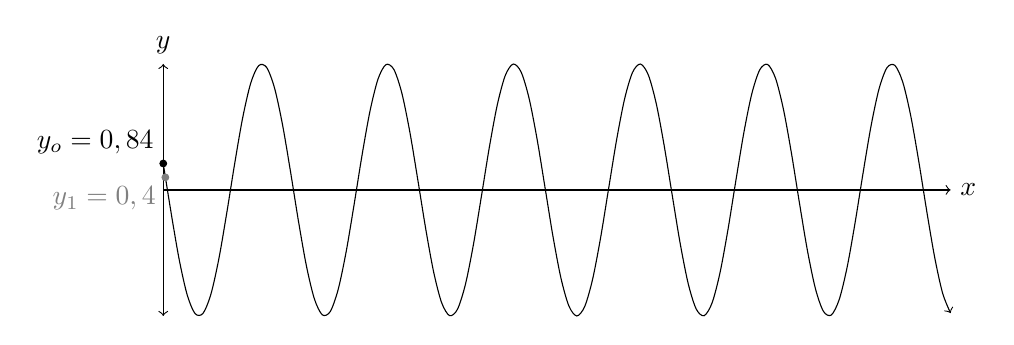
\begin{tikzpicture}[scale=.4,domain=0:25]
      \draw[<->] (0,-4) -- (0,4) node[anchor=south] {$y$};
      \draw[->] (0,0) -- (25,0) node[anchor=west] {$x$};

      \draw[->] plot[samples=100,smooth]({\x},{ 4 * sin( (pi/15 - (\x * pi)/2) r)});
      
      \draw[fill] (0,0.84) circle (3pt) node[anchor=south east]{$y_o = 0,84$};
      \draw[fill,gray] (0.067,0.4) circle (3pt) node[anchor=north east]{$y_1 = 0,4$};
    \end{tikzpicture}
  \]
  \newpage

  2) Imagine uma onda transversal se propagando em uma corda no sentido positivo
   do eixo x a uma velocidade de 60 m/s, cuja amplitude da onda é de 600 cm.
   Sabendo que a sua fase inicial é $\phi = \dfrac{\pi}{2}$
  \vspace*{.2cm}

  \(
    \left\{
      \begin{array}{ccl}
        V_x & = & 60\ \text{m/s} \\
        y_m & = & 600\ \text{cm} = 6\ \text{m}\\
        \phi & = & \dfrac{\pi}{2}
      \end{array}
    \right.
  \)
  \vspace*{.5cm}

  a) Qual o número da onda, sabendo que o comprimento de onda é $\lambda = 7$ mm.
  \[
      k = \frac{2\pi}{\lambda} = \frac{2\pi}{0,007\ \text{m}} = \frac{2.000\pi}{7} \approx 285,71\pi\ \text{rad/m}
  \]

  b) Imaginando que a partícula leva 3 segundos para sair da sua posição máxima transversal, até seu primeiro ponto mínimo.
  Qual é o período da onda? \\
  Precisa-se calcular o tempo entre 2 pontos máximos, como foi de $y_m$ até $-y_m$ fora contado metade do tempo.

  \[
    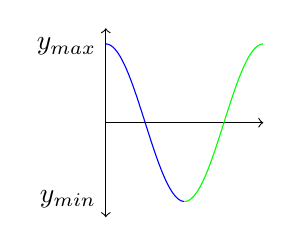
\begin{tikzpicture}[samples=100,smooth]
      \draw[<->] (0,-1.2) node[anchor=south east]{$y_{min}$} -- (0,1.2) node[anchor=north east]{$y_{max}$};
      \draw[->] (0,0) -- (2,0);

      \draw[blue] plot[domain=0:1](\x,{cos(pi * \x r)});
      
      \draw[green] plot[domain=1:2](\x,{cos(pi * \x r)});
    \end{tikzpicture}
  \]

  \[
    T = 2\cdot3 = 6\ \text{s}
  \]

  c) Qual a frequência em Hertz?
  \[
    f = \frac{1}{T} = \frac{1}{6} = 0,1\bar{6}\ \text{Hz}
  \]

  d) Qual a frequência angular?
  \[
    \omega = \frac{2\pi}{T} = \frac{2\pi}{6} = 0,\bar{3}\pi\ \text{rad/s}
  \]

  e) Sabendo que, no tempo $t = 3$ s a partícula apresenta a velocidade transversal
  de $6$ m/s. Qual a posição da partícula nessas condições? \\
  Deixei em fração por pura preferência:
  \[
    y_m(x,t) = 6\cdot\sin\left[\frac{2.000\pi}{7}(x) - \frac{\pi}{3}(t) + \frac{\pi}{2}\right]\ \text{m}
  \]

  Fazendo a parcial no tempo para descobrir a velocidade:
  \[
    V_x(x,t) = -\frac{\pi}{3}\cdot6\cdot\cos\left(\frac{2.000\pi}{7}(x) - 
    \frac{\pi}{3}(t) + \frac{\pi}{2}\right)\ \text{m/s}
  \]

  Que nos dá:
  \[
    V_x(x,t) \approx -6,28\cdot\cos\left[\frac{2.000\pi}{7}(x) - \frac{\pi}{3}(t) + \frac{\pi}{2}\right]\ \text{m/s}
  \]

  Substituindo:
  \[
    6 = -6,28\cdot\cos\left[\frac{2.000\pi}{7}(x) - \frac{\pi}{3}(3) + \frac{\pi}{2}\right]
  \]
  \[
    -0,95 = \cos\left[\frac{2.000\pi}{7}(x) - \pi + \frac{\pi}{2}\right]
  \]

  Aplicando $\cos^{-1}$ conhecido como arco cosseno temos a seguinte equação:

  \[
    2,824 \approx \left(\frac{2.000\pi}{7}(x) - \frac{\pi}{2}\right)
  \]

  Isola x e teremos o resultado:
  \[
    x = \left( 2,824 + \frac{\pi}{2}  \right) \left( \frac{7}{2.000\pi} \right)
  \]
    
  Tacando na calculadora:
  \[
    x \approx 0,0049
  \]

  Isso se não errei nada.
  \vspace*{1cm}
    
    f) Qual a equação da onda?
    \[
      y_m(x,t) = 6\cdot\sin\left[\frac{2.000}{7}\pi(x) - \frac{\pi}{3}(t) + \frac{\pi}{2}\right]\ \text{m}
      \]
      
    g) Qual a equação da velocidade transversal da onda?
    \[
      V_x(x,t) = -2\cdot\cos\left[\frac{2.000\pi}{7}(x) - \frac{\pi}{3}(t) + \frac{\pi}{2}\right]\ \text{m/s}
    \]
      
    h) Elabore um gráfico da onda no ponto $x=1$ m, em função do tempo.
    \[
      y_m(1,t) = 6\cdot\sin\left[\frac{2.000}{7}\pi - \frac{\pi}{3}(t) + \frac{\pi}{2}\right]\ \text{m}
    \]

    

    \[
      \begin{tikzpicture}
        
      \end{tikzpicture}
    \]

    i) Elabore o gráfico da velocidade da onda no ponto x=1 m, em função do tempo.

\end{document}